\chapter{Claim segmentation}
\label{chap:claim_segmentation}

In part~\ref{part:unstruc} of the thesis, we have explored unstructured
approaches to solving argumentation mining problems.  The term unstructured
describes how we approached the tasks of claim clustering
(Chapter~\ref{chap:argclu}), prominent claim identification
(Chapter~\ref{chap:argrec}), and inferring implicit claims
(Chapter~\ref{chap:deriving_implicit}).  For example, in claim clustering we
end up with clusters of claims that express similar arguments.  However, apart
from the vague notion of similarity, we do not have any additional information
to describe the relationships between the clustered claims. Looking at pairs of
similar claims, one claim may be more general than another (i.e., stating that
\emph{all drugs should be banned} is more general than stating \emph{marijuana
is a drug that should be banned}), one claim may involve personal judgements or
call upon factual sources (\emph{I believe marijuana is bad for your mental
health} vs.  \emph{Science confirmed marijuana actually causes mental health
problems}), etc.  Additionally, using unstructured approaches showed that
determining implicit thoughts and opinions proved extremely difficult. Even
when implicit claims were correctly established (mostly through some downstream
task), there was no way to derive the explanation behind the (correct)
selection process. To overcome challenges observed in unstructured
argumentation mining, we turn to structured approaches. 
We start by breaking down a comment into several claims. Then, to 
get a better understanding of the claim, propose a structure for the claim.
The claim structure is formed on a sub-claim level. Finally, structured
claims are then used for argumentation analysis one could not make using
unstructured methods.
As done in previous chapters, we work with argumentative comments from internet
discussions.

We wish to split the user discussion comments into \emph{atomic units
that convey a single thought} -- \textbf{claims}.
The term claim is used to refer to an elementary \emph{argument component}, 
which are a generalization of elementary discourse units
\citep{winter1982towards, givon1983topic, polanyi1996linguistic}
(argumentative units are 
explained in Subsection~\ref{subsec:arg_comp_ext}). Claims as
defined here are not to be confused with claims from Toulmin's or Freeman's
argument model. Splitting text into argumentative claims is important
because of two main reasons. 
First, non-argumentative content is discarded as it does not 
make statements relevant to the topic
(even though sometimes that can prove useful as shown by 
\citep{madnani2012identifying}).
Second, the process of claim segmentation results in claims, which are the
basis of subsequent argumentation analysis. Extracted claims can then be related to each
other (i.e., \pro{support} or \con{attack} relations in Freeman's model),
further categorized to
fit an argument model (i.e.~claims are classified into warrants or rebuttals
in the Toulmin argument framework), directly analyzed (i.e., clustered as
done in Chapter~\ref{chap:argclu}), or structured (i.e., as microstructures or
ontological formalizations as explained in Chapter~\ref{chap:formalization}).

This chapter introduces structured argumentation mining of claims with claim
segmentation. First, we  describe the dataset of claims in
Section~\ref{sec:claim_seg_data}. Next, we will explore different options to
formulate the problem of claim segmentation in
Section~\ref{sec:claim_seg_problem}. After formalizing the claim segmentation
problem, we propose models to solve the claim segmentation problem in
Section~\ref{sec:claim_seg_model}.  Finally, the proposed models are evaluated in
Section~\ref{sec:claim_seg_experiment}.  

\section{Data}
\label{sec:claim_seg_data}

\setlength{\tabcolsep}{4pt}

\begin{table*}[t]
\begin{center}
{\footnotesize
	\begin{tabular}{@{}p{0.2\linewidth} p{0.30\linewidth} p{0.30\linewidth} }
\toprule
\textbf{User comment} & \textbf{Claim segment} & \textbf{Claim paraphrase}   \\
\midrule
\multirow{3}{*}{\parbox{3cm}{
		\emph{Men should fall in love with women that's why they where
		created and women should get married to men because it makes
		everything easier. }
}}
&  
\emph{Men should fall in love with women.}
& \emph{People of opposite sex should fall in love.}
\\
\cmidrule{2-3}
& \emph{that's why they where created} & \emph{Men and women are created to pair.}
 \\
\cmidrule{2-3}
& \emph{women should get married to men because it makes everything easier.} & 
 \emph{Heterosexual marriages make everything easier.}
 \\
 \bottomrule
\end{tabular}}
\end{center}
\caption{An example of a user comment segmented into three claim segments with
	their corresponding paraphrase.}
\label{tab:claim_seg_post_segments}
\end{table*}

We again adopt the dataset of \citet{hasan2014you}, which contains 
user comments from internet two-sided discussions on a number of issues. 
We consider two topics: ``\emph{Gay Rights}'' and 
``\emph{Marijuana}'' and 
sample 100 comments (50 \pro{pro} and 50 \con{con}) from each topic. 
For both topics, we hired trained annotators.
First, annotators segment out claims from user comments.
Second, after segmenting out a claim, the annotators provide a paraphrased
version of the claim.
We assume that paraphrasing helps understanding of claims and will prove useful
in contextualizing claims. 
% TODO think how to incorpore wyner 
% Our work is similar to \citep{wyner2016working} who use a controlled language 
% for paraphrasing claims. 

Claim segmenting separates argumentative from non-argumentative content. 
There are many ways a comment can be segmented into claims in addition to being
a number of ways to paraphrase a claim. 
The ambiguity can be reduced by doing these two tasks jointly. 
The end result paraphrased should be \emph{simplifying claim paraphrases}: 
paraphrases that provide the essence of claims devoid of 
superfluous words and phrases. 
To that end, we adopt nine paraphrasing principles: 
\begin{enumdescript}[leftmargin=!,labelwidth=\widthof{\bfseries Argumentativeness bla}]
\item[Argumentativeness] only argumentative text should paraphrased;
\item[Atomicity] a claim should convey a single thought; 
\item[Authority] experts in claims from expert opinion should be made
	explicit in the paraphrase; 
\item[Brevity] paraphrases should keep only the relevant argumentative
	content; 
\item[Canonicity] canonical terms and phrases are proffered over idiomatic
	language; 
\item[Contextually] claims should be paraphrased by considering their
	local and topical context as well as their context; 
\item[Declarativity] paraphrases should be in declarative form; 
\item[Dereferencing] pronouns and nominal references should be resolved; and
\item[Explicitness] only explicitly stated information should be
	paraphrased, and not whatever might be implied by the claim.
\end{enumdescript}
Unlike most previous approaches to detecting argument component boundaries, we
allow for both overlapping and discontiguous segments. 
 Full annotation guidelines
are in Appendix~\ref{sec:argseg_annotation}. The annotation for ``\emph{Gay Rights}''
was carried out by one trained annotator and took 25 hours.
The annotation for ``\emph{Marijuana}'' was carried out by three annotators. 
The 100 user comments yield 920 claim segments for ``\emph{Gay Rights}'', as did the 100 
user comments in ``\emph{Marijuana}''. 
For the ``\emph{Gay Rights}'' topic, the segments covered 79.6\% of the text,
while the remaining 20.4\% may be considered non-argumentative. The
``\emph{Marijuana}'' topic contained 
more argumentative text, as 88.98\% of text is covered by argumentative 
segments, while 11.02\% was annotated as non-argumentative. 
Table~\ref{tab:claim_seg_post_segments} gives an example of a comment from
the ``\emph{Gay Rights}'' topic split into segmented and paraphrased claims. 
Allowing for overlapping and discontiguous segments offers better coverage,
since a fair number (19.1\% in our dataset) of claims are overlapping or discontinuous.

% \noindent - dataset statistics \\
% - how many examples are overlapping \\

\section{Problem Formulation}
\label{sec:claim_seg_problem}

% \begin{table}
% \small{
% \centering
% \begin{tabular}{c| c c}
%  i & $x_i$ & $Y_i$ \\
% \midrule
%  1& marijuana & $\{1 \}$ \\
%  2& is & $\{ 1 \}$ \\
%  3& believed &  $\{ 1 \}$ \\
%  4& to& $\{ 1 \}$ \\
%  5& be& $\{ 1 \}$ \\
%  6& a& $\{ 1 \}$ \\
% 7 & stepping& $\{ 1 \}$ \\
% 8 & -& $\{ 1 \}$
% \end{tabular}
% \hfill
% \begin{tabular}{c | c c}
%  i & $x_i$ & $Y_i$ \\
% \midrule
% 9 & stone& $\{ 1 \}$ \\
% 10& drug& $\{ 1 \} $ \\
% 11& that& $\{2, 3, 4\}$ \\
% 12& can& $\{2, 3, 4\}$ \\
% 13& eventually& $\{2, 3, 4\}$ \\
% 14& lead& $\{2, 3, 4\}$ \\
% 15& to& $\{2, 3, 4\}$ \\
% 16& addiction& $\{2, 3, 4\}$ \\
% \end{tabular}
% \hfill
% \begin{tabular}{c| c c}
%  i & $x_i$ & $Y_i$ \\
% \midrule
% 17 & to& $\{2, 3, 4\}$ \\
% 18 & heroin & $\{ 2 \}$ \\
% 19 & , & $\{2\}$ \\
% 20 & cocaine& $\{3 \}$ \\
% 21 & and& $\{ \}$ \\
% 22 & other& $\{ 4 \} $\\
% 23 & harder& $\{ 4 \} $\\
% 24 & drugs& $\{ 4 \} $\\
% \end{tabular}
% }
% \caption{An example comment from the ``\emph{Marijuana}'' topic. Each token of
% 	the comment is assigned a set of labels. Segments $2, 3, 4$ overlap on
% 	tokens 10-17.  Segments $3$ and $4$ are discontiguous.}
% \label{tab:multi-label_segment_example}
% \end{table}

% Now, since the dataset is defined, we will mathematically formalize this
% problem.  Let $x = (x_1, \dots, x_N)$ represent a sentence of size $N$
% as a vector of tokens where the index $i$ represents the position of the token in
% the sentence.  Then $\mathbf{Y} = (Y_1, \dots, Y_N)$ is a vector where each
% element represents a set of labels.  Each $Y_i, i \in \{1, \dots, N\}$ is a set
% of labels corresponding to the token $x_i$ at index $i$. The \textbf{claim segmentation}
% problem is then defined as finding function $f$ that maps $\mathbf{x}$ to $\mathbf{Y}$.

A single sentence may contains several claims and, vice versa, a single claim
can span several sentences. For this reason we need to segment the text in
claims. More formally, let
$x = (x_1, \dots, x_N)$ represent text of length $N$
as a vector of tokens where the index $i$ represents the position of the token in
text. Then $Y = (Y_1, \dots, Y_K)$ is a vector where each
element represents a tuple of $N$ elements for $K$ segments. 
$Y_k$ is a tuple
of $N$ values $Y_k = (Y_{k, 1}, \dots, Y_{k, N}),  k \in \{1, \dots, K\}$, where 
value $Y_{k, i} \in \{0, 1\}$ indicates if token $x_i$ is a part of segment $k$. 
The \textbf{claim segmentation}
problem is then defined as finding function $f$ such that 
%$f: \overrightarrow{\mathbf{x}} \to \overrightarrow{\mathbf{Y}}$
$f: \mathbf{x} \to \mathbf{Y}$, where $\mathbf{x}$ and $\mathbf{Y}$
represent the sets of texts and corresponding segments. 
The $k$-th claim segment of $x$ is then defined as 
$\mathbf{\mathit{seg}}_{k} = 
(x_i | f(x)_{k, i} = 1, i \in \{1, \dots, N\})$.
As an example, consider the comment:
\begin{quote}
``\textit{Marijuana is believed to be a stepping-stone drug that
can eventually lead to addiction to heroin cocaine and other harder
drugs}''
\end{quote}
This comment contains 24 tokens, represented as 
$x = \{\textit{Marijuana}, \textit{is}, \textit{believed}, \dots, \textit{drugs}\}$. 
The comment should be segmented into four claims:
\begin{enumerate}
\item ``\emph{Marijuana is believed to be a stepping-stone drug}'', 
\item ``\emph{that can eventually lead to addiction to heroin}'',
\item ``\emph{that can eventually lead to addiction to cocaine}'', and
\item ``\emph{that can eventually lead to other harder drugs}''.
\end{enumerate}
which corresponds to output vector
\begin{align*}
	\mathbf{Y} = (&(1, 1, 1, 1, 1, 1, 1, 1, 0, 0, 0, 0, 0, 0, 0, 0, 0, 0, 0, 0, 0, 0, 0, 0, 0, 0, 0, 0, 0, 0, 0, 0) \\
	 &(0, 0, 0, 0, 0, 0, 0, 0, 1, 1, 1, 1, 1, 1, 1, 1, 0, 0, 0, 0, 0, 0, 0, 0, 0, 0, 0, 0, 0, 0, 0, 0),  \\
	 &\dots)
\end{align*}
The corresponding segments are 
\begin{align*}
seg_1 &= \{\textit{Marijuana}, \textit{is}, \textit{believed}, \dots\, \textit{drug}\},  \\
seg_2 &= \{\textit{that}, \textit{can}, \textit{eventually}, \dots, \textit{heroin}\}, \\
seg_3 &= \{\textit{that}, \textit{can}, \textit{eventually}, \dots, \textit{cocaine}\}, and \\
seg_4 &= \{\textit{that}, \textit{can}, \textit{eventually}, \dots, \textit{drugs}\}
\end{align*}

% As an example, the
% comment (from the ``\emph{Marijuana}'' topic):
% \begin{quote}
% ``\textit{Marijuana is believed to be a stepping-stone drug that
% can eventually lead to addiction to heroin, cocaine and other harder
% % TODO actually is 25 tokens
% drugs.}''
% \end{quote}
% is tokenized into 24 tokens (tokens are space separated for simplicity reasons). 
% It contains four segments: 
% \begin{enumerate}[label=(\arabic*)]
% \item ``\emph{Marijuana is believed to be a stepping-stone drug}'', 
% \item ``\emph{that can eventually lead to addiction to heroin,}'',
% \item ``\emph{that can eventually lead to addiction to cocaine}'' and
% \item ``\emph{that can eventually lead to other harder drugs}''.
% \end{enumerate}

\begin{figure}[t]
	\centering
\tiny
\begin{tabular}{l | ccccccc cccccccc ccc ccccc}
	& Nothing& can& bring& peace& to& this& world 
&Its& a& great& idea& to& try& and& push& 
for& world& peace 
	& but & it & will & never & happen \\
	\midrule
	\texttt{BIO} & \texttt{B} & \texttt{I} & \texttt{I} &
	\texttt{I} & \texttt{I} & \texttt{I} & \texttt{I} & \texttt{B}&
	\texttt{I} & \texttt{I} & \texttt{I} & \texttt{I} & \texttt{I} &
	\texttt{I} & \texttt{I} & \texttt{I} & \texttt{I} & \texttt{I} &
	\texttt{B} & \texttt{I} & \texttt{I} & \texttt{I} & \texttt{I} \\
	\midrule
	\multirow{3}{*}{BR} & 1 & 1 & 1 & 1 & 1 & 1 & 1 
	& 0& 0 & 0 & 0 & 0 & 0 & 0 & 0 & 0 & 0 & 0 
	& 0 & 0 & 0 & 0 & 0 \\

	& 0 & 0 & 0 & 0 & 0 & 0 & 0 
	& 1& 1 & 1 & 1 & 1 & 1 & 1 & 1 & 1 & 1 & 1 
	& 0 & 0 & 0 & 0 & 0 \\

	& 0 & 0 & 0 & 0 & 0 & 0 & 0 
	& 0& 0 & 0 & 0 & 0 & 0 & 0 & 0 & 0 & 0 & 0 
	& 1 & 1 & 1 & 1 & 1 \\

\end{tabular}
	\caption{Binary relevance Multi-label (BR) and \texttt{BIO} labelling
	of comment with three segments: 
	``\textit{Nothing can bring peace to this world}'', 
	``\textit{Its a great idea to try and push for world peace}'', and
	``\textit{but it will never happen}''. 
}
\label{fig:segment_example_bio_multi-label}
\end{figure}

Mapping $\mathbf{x}$ to $\mathbf{Y}$ can be framed as multi-label
classification, since each $Y \in \mathbf{Y}$ can contain up to $N$ labels,
yielding a total of $2^{N}$ possible combinations per element.  Thus, we frame
claim segmentation as multi-label classification (solving multi-label
classification problems is described in Section~\ref{sec:chain_classification}).  
One option to approach the multi-label
classification setup is to apply the binary relevance (BR) setup, but binary
relevance requires searching through an exponential number of solutions.  The
last three rows  of Fig.~\ref{fig:segment_example_bio_multi-label} show BR
labeling of the segments for the example comment. 

As an alternative to inefficient BR labeling various other approaches have been
explored in the context of sequence prediction. 
Extracting sequences has been investigated in information extraction, 
more specifically in the context of 
shallow parsing \citep{sha2003shallow} and named entity
recognition \citep{nadeau2007survey}. \citet{sha2003shallow}
employed \texttt{BIO} encoding for shallow parsing and used conditional random
fields in one of the first structured prediction approaches in information
extraction. \texttt{BIO} labels indicate whether the word is outside a segment
(\texttt{O}), starts a segment (\texttt{B}) or continues a segment
(\texttt{I}). In order to apply \texttt{BIO} labeling, the final segments
\emph{must} be non-overlapping and contiguous. 
Row two in Fig.~\ref{fig:segment_example_bio_multi-label} shows a
comment from the ``Marijuana'' topic 
containing three segments labeled with \texttt{BIO} tags. 
Using \texttt{BIO} tags instead of applying the multi-label approach
simplifies solving the sequence extraction by 
having to predict only a single label per token, which makes the number of solutions 
%for  $x_i \in x$ 
go down from exponential 
%($Y_i \in \{\emptyset, \{1\},  \{2\}, \{1, 2\},  \dots, \{1, \dots, N\}\}$) 
to linear.
%($Y_i \in \{B, I, O\}$). 
%However, multi-label problems can not always be reduced to the \texttt{BIO} 
%tagset. 

In the case when segments are overlapping or discontiguous using \texttt{BIO}
tags can not be used to bijectively encode segments of labels. 
To tackle overlapping and/or discontiguous segments a number of approaches have been
proposed, mostly
in the area of named entity recognition, particularly on
on datasets such as BioInfer \citep{pyysalo2007bioinfer}. 
\citet{byrne2007nested} proposed a solution for 
extracting non-overlapping contiguous entities which uses
tag n-grams instead of words. Working to also solve 
non-overlapping contiguous entities,
\citet{alex2007recognising} proposed using multiple-layer token tagging. 
\citet{finkel2009nested} treated entity recognition as a parsing task
and adopting common state machine parsing approaches. 
More recently, there has been a renewed interest in solving 
the problem of extracting overlapping and contiguous 
entities as part of the 
the SemEval-2014 analysis of clinical texts competition
\citep{pradhan2014semeval}.
One of the tasks in the SemEval competition was medical named entity
recognition, which involved entities which are both discontiguous and
overlapping.  Out of all submissions, only two systems produced solutions that
could handle both discontiguous and overlapping entities.  The first system,
described in \citep{pathak2014ezdi}, uses a standard \texttt{BIO} tagging
pipelined with SVMs to combine resulting spans. Whereas the second system,
described in \citep{zhang2014uth_ccb}, expands on the regular \texttt{BIO}
tagset. They propose to tag each token with one of \textbf{B}, \textbf{I},
\textbf{O}, \textbf{BD}, \textbf{ID}, \textbf{BH}, and \textbf{IH}, which
denote \textbf{B}eggining of entity, \textbf{I}nside entity, \textbf{O}utside
of entity, \textbf{B}eginning of \textbf{D}iscontigious entity, \textbf{I}nside
of \textbf{D}iscontigious entity, \textbf{B}eginning of \textbf{H}ead, and
\textbf{I}nside of \textbf{H}ead. However, this encoding is lossy, which makes
decoding from tags to segments ambiguous in some cases.  Furthermore, using this
encoding may produce
invalid sequences of tags.  Apart from this work, this expanded \texttt{BIO}
encoding was used in \citep{muis2018learning} where they proposed a
hypergraph-based model to solve the clinical named entity challenge.  A
thorough survey on extracting overlapping and discontiguous named entities can
be found in \citep{dai2018recognizing}. In the survey, the authors consider all
tag encodings and recommend multi-label encoding if feasible, as it is the only
one which is unambigous.

The clinical named entity extraction problem and semantic parsing are
equivalent to the claim segmentation problem. 
Both problems are usually framed as sequence labeling problems. Thus, as an 
alternative to multi-label classification, we also frame 
claim segmentation as a sequence labeling problem. 
We consider the \texttt{BIO} approach since it is unambigous. 

The multi-label approach can handle both discontiguous and overlapping entities,
but requires search through a much broader (exponential) solution space.
On the other hand, the \texttt{BIO} tagging approach has a linear search space,
but applying it can only work in the case of contiguous and non-overlapping segments.
A comparison of the \texttt{BIO} and multi-label token labeling for a comment divided
into claim segments is shown in 
Figure~\ref{fig:segment_example_bio_multi-label}.
% and an example of a comment with overlapping
% and discontiguous segments in shown in table~\ref{tab:multi-label_segment_example}.

\begin{figure}
	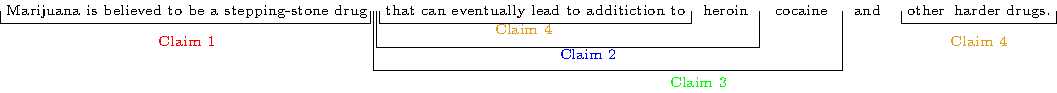
\includegraphics[width=\textwidth]{claim_segmentation_split-figure0.pdf}
	\caption{An example of comment made in the ``Marijuana'' topic. 
	\textcolor{red}{Claim 1} is a regular segment. 
	\textcolor{blue}{Claim 2} and \textcolor{green}{Claim 3} are mutually overlapping.
	\textcolor{orangegreen}{Claim 4} is both overlapping and discontiguous.}
	\label{fig:segment_example_range}
\end{figure}

%'<S1>Marijuana is believed to be a stepping-stone drug
%</S1><S2><S3><S4>that can eventually lead to addiction to
%</S3></S4>heroin,</S2><S3> cocaine</S3> and<S4> other harder
%drugs.</S4>'

% <S1>Nothing can bring peace to this earth.</S1> <S2>Its a great idea to try and
% push for world peace</S2> <S3>but it will never happen...</S3>'

\begin{algorithm}[t]
	\begin{algorithmic}[1]
\Function{is\_punctuation}{ch}
		\If{$ch = ``." \hspace{0.1cm} \cup \hspace{0.1cm} ch = ``?"
		\hspace{0.1cm} \cup \hspace{0.1cm}  ch = ``!"$}
\State
\Return $\mathit{True}$
\Else
\State
\Return $\mathit{False}$
\EndIf
%\Return $out$
\EndFunction

\State
\State 

\Function{na\"ive\_heuristic}{$text$}

	\State $\mathit{seg\_id} \gets 1$
	\State $Y[\mathit{seg\_id}] \gets \emptyset$
	\ForAll{$i \in |\mathit{text}|$}
		\State $token \gets text[i]$
		\State $Y[\mathit{seg\_id}] \gets Y[\mathit{seg\_id}] \cup \mathit{token}$
		\State
		\If{$\mathit{IS\_PUNCTUATION}(\mathit{token}) \cap i \neq 0$}
		\State $\mathit{seg\_id} \gets \mathit{seg\_id} + 1$
		\EndIf
	\EndFor
	\State
	\Return $Y$
\EndFunction
\end{algorithmic}
\caption{Claim segmentation punctuation based heuristic.
Input is a list of tokens, outputs a nested list of lists, where 
each list corresponds to a segment. 
None of the tokens is declared as non-argumentative.
The \texttt{IS\_PUNCTUATION} function has been simplified for readability
purposes, since in practice it uses regular expressions. 
	}
\label{alg:heuristic_claimseg}
\end{algorithm}

\section{Models}
\label{sec:claim_seg_model}

We frame the claim segmentation problem as supervised learning token-level 
classification (as it was done in \citep{ajjour2017unit} to detect
argumentative units of text). 
To label tokens, we use one of two 
token-level tagging solutions. 
First, we adopt the binary relevance multi-label classification (\texttt{BR})
approach, where each token can belong to zero or more claim segments. For the
second (\texttt{BIO}) approach, we discard overlapping and discontiguous
segments and then apply standard \texttt{BIO} labels.  After applying the
tagging to data, we propose three models to solve the claim segmentation
problem. In the first approach, we apply a typical argumentation mining solution
where each sentence is treated as a claim segment. For the second approach 
we use n-gram features as input to a SVM. In the third approach 
we combine deep learning and structured prediction.

\paragraph{Na\"ive Heuristic. } 
Our baseline model is extremely similar to most approaches in argumentation
mining: we declare each sentence of the comment to be a claim.  This approach
is common in argumentation mining with the difference that some sentences may
be declared non-argumentative \citep{rooney2012applying,
stab2014identifying}, which is not the case in our approach.  
We consider this assumption is reasonable, given
that a large portion (>80\%) of the dataset is argumentative.  For each
comment, we simply iterate through all tokens and start a new claim when a
token equals a punctuation mark. This is a similar to sentence segmentation
\citep{palmer2000tokenisation}. The heuristic is outlined in
Algorithm~\ref{alg:heuristic_claimseg}. An example of how the algorithm works
for a comment is shown in Table~\ref{tab:heuristic_example}. This approach
inherently can not extract discontiguous and overlapping segments.

\begin{table}[t]
\begin{tabular}{@{}p{0.5\linewidth} p{0.50\linewidth}}
\toprule
\multirow{7}{*}{
\parbox{7cm}{
\textit{if we legalize pot there wil be a sharp increase in 
demand and consumption over a period of time
then............it will start to decline....slowly at first until
smoking pot becomes drinking wine.......only on special
occasions........... that's why we should continue the war
it's not like weed is damn near impossible to obtain ...... in my
opinion there is no war ....... there never was ...}
}}
		& \emph{if we legalize pot there wil be a sharp increase in 
demand and consumption over a period of time
	then ............} \\ \cline{2-2}
		& \emph{it will start to decline .... } \\ \cline{2-2}
		& \emph{slowly at first until
	smoking pot becomes drinking wine .......} \\  \cline{2-2} 
	& \emph{
only on special
occasions
...........
		} \\  \cline{2-2}
	& \emph{
that's why we should continue the war
it's not like weed is damn near impossible to obtain ......
		} \\\cline{2-2}
	& \emph{
in my
opinion there is no war .......
} \\\cline{2-2}
	& \emph{
there never was ...
} \\
\bottomrule
\end{tabular}
	\caption{An example of how the heuristic algorithm handles input (left column) to produce 
	segmented output (right column). }
\label{tab:heuristic_example}
\end{table}

\paragraph{SVM. } 
We use a weighted SVM, with 
the ratio between classes in the training set used to assign weight values, 
giving classes with less examples more prominence. 
% # We use the token and a configurable-sized context window of surrounding tokens
% # as input to the model. 
For features, we use tf-idf and 
distributed word representations 
(fastText\footnote{https://fasttext.cc/}
and word2vec\footnote{https://code.google.com/archive/p/word2vec/}
pretrained vectors).
Finally, to train the model, we use $5 \times 3$ nested-cross validation
optimizing hyperparameters $C$ and $\gamma$ using
grid-search (model selection described in Section~\ref{sec:selection}).

\paragraph{BiLSTM-CRF Model.}
Finally, we try combining deep learning (BiLSTM) and structured prediction
(CRF). The reason we opt for this model is twofold. First, BiLSTMs have
previously been successfully used in argumentation mining
\citep{habernal2016argument}.  Second, the combination of a BiLSTM with a CRF
is considered an extremely strong baseline (and often proves as a topline) for
sequence tagging problems \citep{huang2015bidirectional}.  The general idea of
a BiLSTM-CRF model is described in Subsection~\ref{subsec:lstm_crf}.  We make a
few minor modifications in our model.  Our model works in two stages. In the
first stage, a BiLSTM is used to encode a sequence of tokens of the comment.
The BiLSTM produces pairs of hidden states and outputs. The outputs of the
BiLSTM are then fed into a feed-forward linear layer which maps the BiLSTM
outputs to the label probability space. In the second stage, the output of the
BiLSTM is used as features for the CRF.  The CRF combines the BiLSTM outputs
with a state transition table of possible tags to efficiently use past and
future tags to predict the current tag. The Viterbi algorithm (described in
Subsection~\ref{sec:viterbi}) is used to efficiently compute optimal tag
sequences. 

The parameters of the BiLSTM-CRF model include 
\begin{enumerate*}[label=(\arabic*)]
\item BiLSTM parameters, 
\item linear layer weights, and 
\item state transition matrix of the CRF. 
\end{enumerate*}
As for the hyperparameters of the model, we use 200 feed forward units, set the
word embedding size to 300, and use a single layer bi-directional LSTM to encode
sequences.  We consider using pretrained word embeddings and training
embeddings from scratch.  Furthermore, we experiment by enabling and disabling
fine-tuning of input embeddings when using pretrained word embeddings.  
We use negative log-likelihood as the loss function. We train
and evaluate the model using 5-fold cross-validation. 

% potencijalno staviti u experiments
%  When experimenting with In the multi-label
%  setup, we attempt to share the transition matrix across different when training
%  across claims.  

\section{Experiments}
\label{sec:claim_seg_experiment}

\begin{algorithm}[t]
\begin{algorithmic}[1]
	\Function{precision\_offset}{$\mathit{predicted}, \mathit{true}, \mathit{offset}$}
\State $\mathit{found} \gets \{\}$
\State
\ForAll{$i \in |\mathit{true}|$}
  \ForAll{$j \in |\mathit{predicted}|$}
	\State $\mathit{common} \gets $\texttt{LCS\_LENGTH}$(\mathit{true}[i], \mathit{predicted}[j])$
	\State
	\State $\mathit{is\_smaller\_than\_offset} \gets |\mathit{predicted}[j]| > \mathit{offset}$
	\State $\mathit{is\_common\_enough} \gets $ $|\mathit{predicted}[j]| -
	\mathit{common} \leq \mathit{offset}$
	\State $\mathit{has\_small\_size\_diff} \gets |\mathit{predicted}[j]| -
	|\mathit{true}[i]| \leq \mathit{offset}$
	\State
	\If{$\mathit{is\_smaller\_than\_offset} \cap 
	\mathit{is\_common\_enough} \cap \mathit{has\_small\_size\_diff}$}
	  \State $\mathit{found} \gets \mathit{found} \cup \mathit{true}[i]$
	  \State \textbf{break}
	\EndIf
  \EndFor
\EndFor
\State 
\State
\Return $\frac{|found|}{|true|}$
\State
\EndFunction
\end{algorithmic}
\caption{Algorithm to calculate precision with arbitrary offset between 
	two sets of segments, each segment being a list of tokens.
	\texttt{LCS\_LENGTH} calculates the length of the 
	longest common subsequence of two sequences.  
	We use a solution presented in
	\citep{hunt1977fast}.
	Recall is equivalently calculated, but with different inputs. 
	}
\label{alg:precision_offset}
\end{algorithm}

We compare the proposed models using two main set of metrics. The first set of 
metrics is standard when evaluating information extraction problems:
precision, recall, and F1-score of the retrieved claims, 
which we denote with P, R, and F1 respectively \citep{hripcsak2005agreement}. 
Also, since we are dealing with sequences, we wish to allow 
for small mistakes. This means that a retrieved claim which
has an extra or missing token will still count as correctly retrieved. 
Algorithm~\ref{alg:precision_offset} shows how to calculate precision with an
configurable margin of error (offset) on the token level.
The measure indicates when the predicted claim is close to the gold one,
since having exact claims might not always be important. For example, the
comment ``\emph{Nothing can bring peace to this earth. Its a great idea to try and
push for world peace, but it will never happen...}'' contains three claims,
one of them being ``\emph{but it will never happen...}'', but if the predicted claim is
``\textit{world peace but it will never happen...}'' and the allowed offset is two or more
this will be counted as correct. 
The reported results use allowed offset of two and denote as lenient precision,
lenient recall, and lenient F1-score as lP, lR, and lF1 respectively.

\begin{table}
	\centering
\begingroup
\setlength{\tabcolsep}{10pt} % Default value: 6pt
\renewcommand{\arraystretch}{1.5} % Default value: 1
	\begin{tabular}{l c  c c c c c c}
\toprule
		Tagset & Model & P & R & F1 & lP & lR & lF1 \\
      \midrule
		& Heuristic    & \textbf{0.41} & 0.23 & 0.29 & 0.89 & 0.49 & 0.63 \\
		\cline{2-8}
		\multirow{2}{*}{\texttt{BR} } & SVM & 0.03 & 0.01 & 0.02 & 0.09 & 0.01 & 0.02 \\
		                     & BiLSTM-CRF & 0.12 & 0.01 & 0.02 & 0.32 & 0.04 & 0.06 \\
		\cline{2-8}
		\multirow{2}{*}{\texttt{BIO}} & SVM & 0.35 & 0.14 & 0.20 & 0.88 & 0.35 & 0.50 \\
				     & BiLSTM-CRF & 
				     \textbf{0.41} & 
				     \textbf{0.27}  & \textbf{0.32} & \textbf{0.92} & \textbf{0.61} & \textbf{0.74} \\
      \bottomrule
	\end{tabular}
	\endgroup
	\caption{Claim segmentation standard and lenient (set offset to two) precision, recall, 
	and F1 score in the \texttt{BR} and \texttt{BIO} setups. }
	\label{tab:claim_seg_results}
\end{table}

\paragraph{Multi-label encoding (\texttt{BR}).} 
First, we wish to compare the three proposed approaches: 
the na\"ive heuristic, the SVM, and the BiLSTM-CRF
in terms of both standard and lenient precision, recall, and F1-score.
In both the SVM and BiLSTM-CRF approach, we use \texttt{BR} encoding. 
In the CRF, we do not share the tag transition table across 
claim segments and train embeddings from scratch.
Results are in Table~\ref{tab:claim_seg_results} with boldfaced
best results. 
The results clearly show that the na\"ive heuristic model significantly outperforms
both the BiLSTM-CRF and the SVM model using \texttt{BR} encoding. 
The results of the heuristic model have
high precision and low recall. One reason may be that 
the model favors longer claims segments (that map to sentences). 
Intuitively, longer sentences contain more claims, on which the 
heuristic model performed poorly. 
The outputs of the SVM and BiLSTM-CRF model predominately include 
the majority labels, so they manage to extract claims in short posts
(consisting of very claims). 
An obvious problem for the SVM and BiLSTM-CRF model 
is not having enough data points  
(100 samples for 48 labels). We considered reusing data across different
labels, but to no significant effect, since most of the training examples were
then labeled differently. More specifically, it would often be the case that
a token would be labelled as a claim in one
training instance, but not in another.
This is a less of a problem when dealing with a task such as named entity
recognition, as the number of such conflicting data points is much smaller. 
This clearly suggests that using the \texttt{BR} encoding struggles to 
predict claims. 
To improve the results, we also attempt to fine tune pretrained embeddings
during training time and share the transition table in the BiLSTM-CRF setup. 
Sharing the CRF
state transiton table (which in this case defines the probability of going from a
non-argumentative to an argumentative state and vice versa) across folds should provide
models stronger priors of when a claim starts or ends. 
However, we do not see any performance improvement in that case either.

\paragraph{\texttt{\textbf{BIO}} encoding.} Since using \texttt{BR} encoding
produces limited results, we explore the \texttt{BIO} encoding. In order to do
so, we first need to label the dataset using \texttt{BIO} tags. Before applying
the \texttt{BIO} tagset, overlapping and discontiguous claims are discarded.
Then, we assign \texttt{BIO} tags to tokens (example in \texttt{BIO} labeling
is shown in Fig.~\ref{fig:segment_example_bio_multi-label}).  To measure the
topline results, we perform the inverse mapping from \texttt{BIO} tags to
claims and compare against gold claims (which include discontiguous and
overlapping claims).  The topline precision, recall, and F1-score are then
$1.0$, $0.74$, and $0.84$ respectively. Using the token and \texttt{BIO} tag
pairs, we now train the SVM and BiLSTM-CRF models.  This time around, we end up
with comparable results with the na\"ive heuristic baseline, as shown in the
final two rows of Table~\ref{tab:claim_seg_results}.  The SVM model performs
0.09 and 0.13 less F1-score percentage points than the na\"ive heuristic, but
much better (0.32 and 0.79 more F1-score percentage points) than the SVM model
using \texttt{BR} encoding.  In terms of F1-score, the BiLSTM-CRF showed the
best performance, narrowly outperforming the na\"ive heuristic by 0.03 and 0.09
F1-score percentage points. 
% The na\"ive heuristic has higher precision, most likely since it produced
% less claim segments (509 versus 565 by the BiLSTM+SVM model). 

Looking at the results in general, predicting the exact boundary of a  claim
segment is a difficult, albeit feasible, task, since the best performing model produced
0.32 F1-score. 
However, the claims produced were often very close to the exactly correct one, 
which is reflected with the 0.74 offset F1-score for the best-performing model. 
Inspecting the predicted labels of all models, none of the models
correctly label non-argumentative segments (\texttt{O} labels). 
The most likely reason lies in the fact that non-argumentative content
is greatly underrepresented in this dataset and we should work on a method to 
such as penalizing or oversampling. 
In general, to solve the claim segmentation problem, the na\"ive
heuristic proved difficult to beat, even by advanced deep learning and
structured prediction techniques.
To further research on claim segmentation, we propose working on slighly more
advanced heuristics as a starting point, as a very simple one produced decent
results. The claim segmentation looks like mostly a syntax-related problem, so
perhaps looking into exploiting syntactic clues would yield even better
results.  In Chapter~\ref{chap:claim_structuring}, we will revisit claim
segmentation as part of a joint model that also structures claims. 

% Now that we
% have scratched the  claim segmentation problem, we move on to the
% next stage in the argumentation mining pipeline: argumentative structure
% prediction. 
% 
% 110 # precision basic 208 509 0.4086444007858546                                                                                                                                                                   
% 111 # recall basic 208 921 0.2258414766558089                                                                                                                                                                      
% 112 # offset 452 509 0.888015717092338                                                                                                                                                                             
% 113 # offset 452 921 0.49077090119435396                                                                                                                                                                           

% # separate classifiers, non shared transitions
% # precision basic 31 288 
% # recall basic 30 921
% 
% # joined classifiers, non shared transitions
% # precision basic 28 203
% # recall basic 27 921

% BiLSTM with adam
% precision basic 251 614 0.40879478827361565
% recall basic 251 921 0.2725298588490771
% offset 565 614 0.9201954397394136
% offset 565 921 0.6134636264929425


% BiLSTM with offset
% # basic 254 641
% # basic 254 921
% # offset 528 838
% # offset 528 921
% 
% # epoch = 25
% # precision 204 / 641
% # recall 204 921



% # SVM BR
% # precision basic 3 99 0.030303030303030304
% # recall basic 3 921 0.003257328990228013
% # offset 9 99 0.09090909090909091
% # offset 9 921 0.009771986970684038

% # SVM BIO
% # precision basic 129 365 0.35342465753424657
% # recall basic 129 918 0.14052287581699346
% # offset 322 365 0.8821917808219178
% # offset 322 918 0.35076252723311546

% \section{Conclusion}
% \label{sec:claim_seg_conclusion}

% In this chapter, we have explored the claim segmentation problem.  We
% constructed a dataset of comments split into claims. The claim segmentation
% problem was then mathematically formalized in two ways: a multi-label
% binary relevance and a \texttt{BIO} encoding setup. The comparison of a
% na\"ive heuristic, SVM, and BiLSTM+CRF model 
% showed that a simple sentence splitting heuristic is a strong baseline to
% detect claims in text. This justifies the approach of most argumentation
% mining literature which assumes claims matches very well to sentences. 
% Additionally, trying to detect discontiguous and overlapping claims proved 
% extremely difficult in all experimental setups. 
% Perhaps starting from a purely structured SVM
% approach proposed by \citet{mcdonald2005flexible} would yield better results.

